\documentclass{homework}
% \usepackage{graphicx} % Required for inserting images
\usepackage{amsmath}
\usepackage{gensymb}
\usepackage{subfig}
\usepackage{float}
\usepackage{pythonhighlight}

\class{APPM 5600}
\title{Homework 3}
\author{Sean Jennings}
\date{September 20, 2024}

\begin{document}
\maketitle

\section{Problem 1}
For the proceeding problems we look at the magnitude of the derivative of 
the iterator $x_{k+1} = f(x_k)$. $|f'(x)| < 1$ in some neighborhood of the
fixed point, if and only if the series $\{x_k\}$ converges.

\begin{letterenum}
\item Let $f(x) = -16 + 6x  + 12 / x$, so that $x_{k+1} = f(x_k)$. Since the
derivative of $f$ is:
\begin{equation*}
    f'(x) = 6 - 12 / x^2
\end{equation*}
at $x=x^*=2$ we have $f'(x^*) = 3$. Thus, $f'$ is continuous, there is some neighborhood $E$
of the fixed point where $|f'(x)| > 1$ for all $x \in E$. Thus, $f$ is not a contraction on
$E$ and the series does not converge.

\item Let $f(x) = 2/3 x + 1/ x^2$. Then, the derivative is given by:
\begin{equation*}
    f'(x) = 2/3 - 2 / x^3
\end{equation*}
which evaluates at the fixed point $x^* = 3^{1/3}$ to $f'(x^*) = 0$. $\{x_k\}$ converges
to $x^*$ for $x_0$ sufficiently close to $x^*$.

To check the order of convergence, we look at the Taylor series expansion around $x^* = 3^{1/3}$.

\begin{equation*}
    f(x) = f(x^*) + f'(x^*) (x - x^*) + \frac{f''(\eta)}{2} (x - x^*)^2
\end{equation*}
for some $\eta$ between $x^*$ and $x$. Then, we have
\begin{equation*}
    e_{k+1} = |x_{k+1} - x^*| = | f(x_k) - f(x^*)| = \frac{f''(\eta)}{2} e_k^2
\end{equation*}
since $f'(x^*) = 0$. Letting $C = \max_{\eta}\{f''(\eta)/2\}$ over $\eta$ between $x^*$ and $x_0$,
we see that $e_{k+1} \leq C e_k$ so that convergence is quadratic.

\item With $f(x) = 12 / (1 + x)$, we have
\begin{equation*}
    f'(x) = - \frac{12}{(1+x)^2}
\end{equation*}
and $|f'(x^*)| = 3/4 < 1$. Thus, the iteration $x_{k+1} = f(x_k)$ converges. The first order
Taylor expansion around $x^* = 3$ gives:
\begin{equation*}
    f(x) = f(x^*) + f'(\eta) (x - x^*)
\end{equation*}
for some $\eta$ between $x^*$ and $x$. Then, in the limit as $k\to\infty$, we have $\eta \to x^*$,
so that:
\begin{equation*}
    \lim_{k\to\infty} \frac{e_{k+1}}{e_k} = \lim_{k\to\infty} \frac{|f(x) - f(x^*)|}{|x - x^*}
        \leq \lim_{k\to\infty} \biggl| f'(\eta)\biggr| = f'(x^*) = 3/4
\end{equation*}
Thus, the convergence is linear with rate 3/4.

\end{letterenum}

\section{Problem 2}
\begin{letterenum}
\item Put $t_0 = 60$ days into the equation for temperature, and find the $x$ such that
$T(x, t_0) = 0$. Therefore we have:
\begin{equation*}
    \frac{-T_s}{T_i - T_s} = \text{erf} \biggl(\frac{x}{2\sqrt{\alpha t_0}}\biggr)
\end{equation*}
We add by the constant on the left hand-side and define the right side of the this equation 
to be $f$.
\begin{equation*}
    f(x) = \text{erf} \biggl(\frac{x}{2\sqrt{\alpha t_0}}\biggr) + \frac{T_s}{T_i - T_s}
\end{equation*}

Then, the root of $f$ is the distance at which the pipe will freeze after 60 days. Taking
the derivative yields:
\begin{equation*}
    f'(x) = \frac{2}{\sqrt{\pi}} \exp \biggl(- \frac{x^2}{2 \alpha t_0} \biggr)
\end{equation*}
A plot of $f$ is in Figure \ref{fig:f-vs-x}.

\begin{center}
    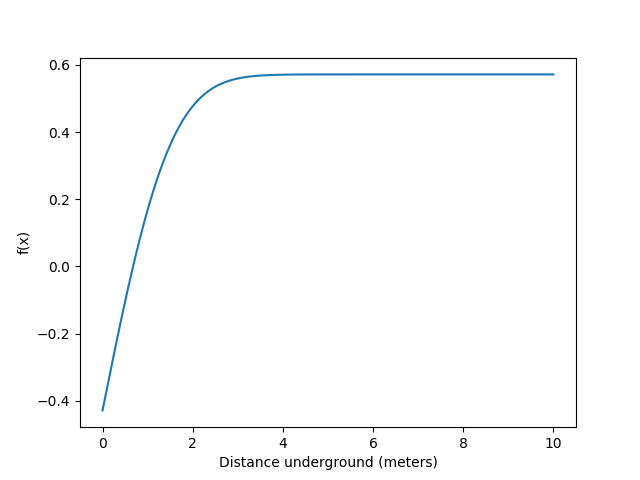
\includegraphics[width=0.5\linewidth]{Images/temp_plot.png}
    \captionof{figure}{f(x) on interval [0, $\bar{x}$] with $\bar{x} = 10$}
    \label{fig:f-vs-x}
\end{center}

\item With the bisection algorithm, we find a root of $x^* = 0.6769618544819167$.
\item With the newton algorithm and initial guess $x_0 = 0.01$, we find a root of
$x^* = 0.6769618544818856$. With $x_0 = \bar{x} = 10$ Newton's method fails because
$f'(x)$ is close to 0. This can be seen by the very flat slope on the right side of
the plot in figure \ref{fig:f-vs-x}. The preferred method would depend on the context
of the function to be evaluated. While Newton's method converges faster, bisection
may be useful in cases where the derivative is hard to evaluate, close to 0, or the
root has high (and unknown) multiplicity.

\end{letterenum}

\section{Problem 3}
\begin{letterenum}
\item Let $f(x) = (x - \alpha) (x - \beta) (x - \gamma)$. Then,
\begin{align*}
    f'(x) &= (x - \beta)(x - \gamma) + (x - \alpha) (x - \gamma) + (x - \alpha) ( x- \beta) \\
        &= (x - \gamma) (2x - (\beta + \alpha)) + (x - \alpha) (x - \beta)
\end{align*}

Evaluating at $x_0 = (\alpha + \beta) / 2$, we have
\begin{equation*}
    f'(x_0) = (x_0 - \alpha) ( x_0 - \beta)
\end{equation*}
since $2x_0 - (\alpha + \beta) = 0$. Thus, the first step of newton's method
yields:
\begin{equation*}
    x_1 = x_0 - \frac{f(x_0)}{f'(x_0)} = x_0 -
        \frac{(x_0 - \alpha)(x_0 - \beta)(x_0 - \gamma)}{(x_0 - \alpha)(x_0 - \beta)} = \gamma
\end{equation*}

\item See figure \ref{fig:same-roots} for an illustration of when the roots coincide with $\alpha < \beta = \gamma$ and $f'(\alpha) > 0$.
All other cases follow from symmetry.

When two of the roots coincide, there will be one point $x_f$ where the slope
of $f$ is zero. Newton's method will fail at the point. For any initial point $x_0$ with
$x_0 < x_f$, the tangent line will intersect the $x$-axis to the left of $\alpha$
since the curve $f$ is concave down in this section. Therefore, if $x_0 < x_f$, $x_n < x_f$
for all $n\geq0$.

\begin{center}
    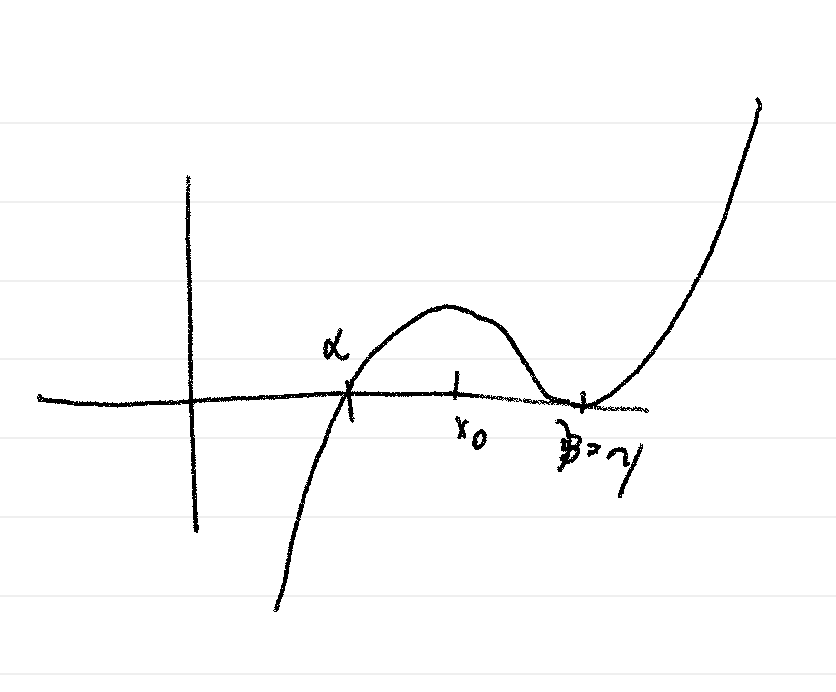
\includegraphics[width=0.5\linewidth]{Images/same_roots.png}
    \captionof{figure}{Cubic polynomial with $\beta = \gamma$}
    \label{fig:same-roots}
\end{center}

For $x_f < x_0 < \beta$, the slope of the tangent line is negative and $f(x_0) > 0$, so
we will have the x-intersect to the right of $x_0$. That is, $x_1 > x_0 > x_f$. If $x_0 > \beta$
the tangent line will intersect the x-axis to the right of $\beta$ since $f$ is concave up
in this region. Again, $x_0 > x_f$ implies that $x_n > x_f$ for all $n\geq 0$.

Thus, the regions $E_1 = \{x | x > x_f\}$  and $E_2 = \{x | x < x_f\}$ are invariant
under Newton's method and (assuming that they converge) they correspond to the basin
of attraction for roots $\beta = \gamma$ and $\alpha$, respectively.

\item Figure \ref{fig:different-roots} shows the case where the roots are unique.

Assume $\alpha < \beta < \gamma$. By a similar argument to part (b), any initial point with
$x_0 < \alpha$  (or $x_0 > \gamma$) will remain less than $\alpha$ ($>\gamma$). However,
there are now two points with slope of 0, $x_{f,1}$ and $x_{f,2}$. Since the intersection
of the tangent line approaches $+\infty$ as $x_0 \to (x_{f,1})$ from the positive side,
and the intersect approaches $-\infty$ as $x_0 \to (x_{f,2})$ from the negative side,
$x_1$ can take any real number. To each $x_{f,1}$ there corresponds a starting guess $x_0$
in the interval $I_f = [x_{f,1}, x_{f,2}]$ with $x_1 = x_{f,1}$. Thus, $x_0$ will also lead to
failure. But by an iterative argument there is another point such that $x_{f,1}$ will be reached
in 2 steps, and a third point where the failure point will be reached in 3 steps. All these
points must be unique (otherwise it would have failed at an earlier step!) and therefore
there is an infinite number of points in the interval $I_f$ which will fail to converge
to a root.

\begin{center}
    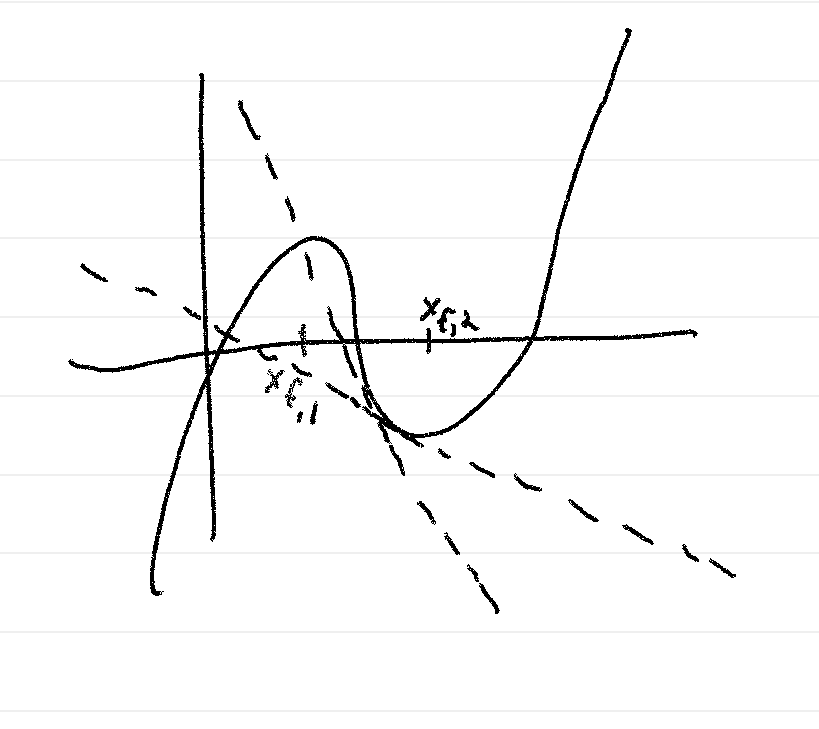
\includegraphics[width=0.5\linewidth]{Images/different_roots.png}
    \captionof{figure}{Cubic polynomial with unique roots}
    \label{fig:different-roots}
\end{center}

\




\end{letterenum}

\section{Problem 4}
\begin{letterenum}
\item The derivative of $f(x) = (x - x^*)^p q(x)$ is
\begin{equation}
    f'(x) = (x - x^*)^p q'(x) + p (x - x^*)^{p-1} q(x)
\end{equation}

Let $g(x) = x - f(x) / f'(x)$. Then,  $x_{k+1} = g(x_k)$. Plugging in The
expression for $f(x)$ we have:
\begin{equation*}
    g(x) = x - \frac{(x - x^*) q(x) }{(x - x^*) q'(x) + p q(x)}
\end{equation*}
Taking the derivative yields:
\begin{equation}
    g'(x) = 1 - \frac{q(x)}{(x- x^*) q'(x) + p q(x)} - (x - x^*)\frac{d}{dx} \biggl(
        \frac{q(x)}{(x - x^*) q'(x) + p q(x)}
    \biggr)
    \label{eq:g}
\end{equation}

So that the derivative at $x = x^*$ is given by $g'(x^*) = 1 - 1/p$. Since $|g(x^*)| < 1$
for $p>0$, $g$ is a contraction and therefore converges in some neighborhood of $x^*$.

A first order Taylor expansion of $g$ gives:
\begin{equation}
    g(x_k) = g(x^*) + g'(\eta) (x_k - x^*)
\end{equation}
for some $\eta$ between $x_k$ and $x^*$. Thus,
\begin{equation*}
    \lim_{k\to\infty} \frac{|x_{k+1} - x^*|}{|x_k - x^*} 
        \lim_{k\to\infty} \frac{|g(x_k) - g(x^*)|}{|x_k - x^*} 
        \leq \lim_{k\to\infty} |g'(\eta)| = g'(\alpha) = \frac{p-1}{p}
\end{equation*}
Therefore, the iteration $x_{k+1} = g(x_k)$ converges linearly with a rate $(p-1)/p$.

\item Let $h(x) = x - p f(x) / f'(x)$. As we saw in problem 1(b), to show that
the series generated by $x_{k+1} = h(x_k)$ converges quadratically, it is sufficient
to show that $h'(x^*) = 0$. But since $h$ and $g$, the second term is multiplied
by a factor of $p$. In an analogous derivation to equation (\ref{eq:g}), with
a factor of $p$ multiplying the second term shows that $g'(x^*) = 1 - p * (1 / p) = 0$.
Therefore, the modified Newton method converges quadratically, which is equivalent
to the statement that there exists $C$ for which
\begin{equation*}
    e_{k+1} \leq C e_k^2
\end{equation*}
for all $k\geq 0$.

\item Figures \ref{fig:error-newton} and \ref{fig:error-modified} show the error
tables for the standard and modified Newton's methods respectively. Plots are shown
in figures \ref{fig:error-plot-newton} and \ref{fig:error-plot-modified}. Generally,
the theory and code line up nicely. However, for the modified Newton's method
on the 5th iteration it reaches within machine precision of the true root
while the change between steps $|x_{k+1} - x_k|$ is still greater than the desired
tolerance of 1e-15. This causes a division by zero error because the derivative evaluates
to zero, even though the root has been successfully found.

\begin{center}
    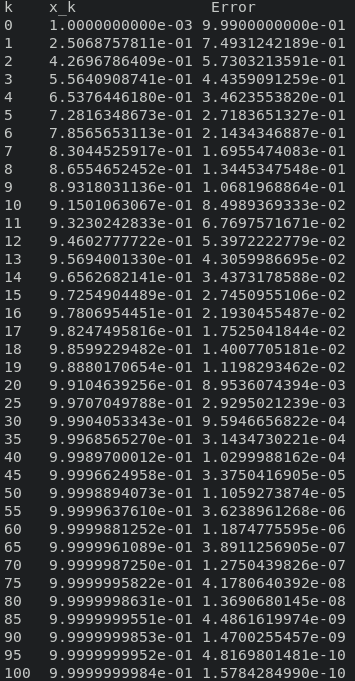
\includegraphics[width=0.5\linewidth]{Images/error_table_newton.png}
    \captionof{figure}{Errors for standard Newton's method on $(x-1)^5 e^x$}
    \label{fig:error-newton}
\end{center}
\begin{center}
    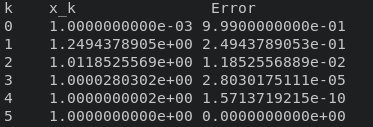
\includegraphics[width=0.5\linewidth]{Images/error_table_modified.png}
    \captionof{figure}{Errors for modified Newton's method on $(x-1)^5 e^x$}
    \label{fig:error-modified}
\end{center}

\begin{center}
    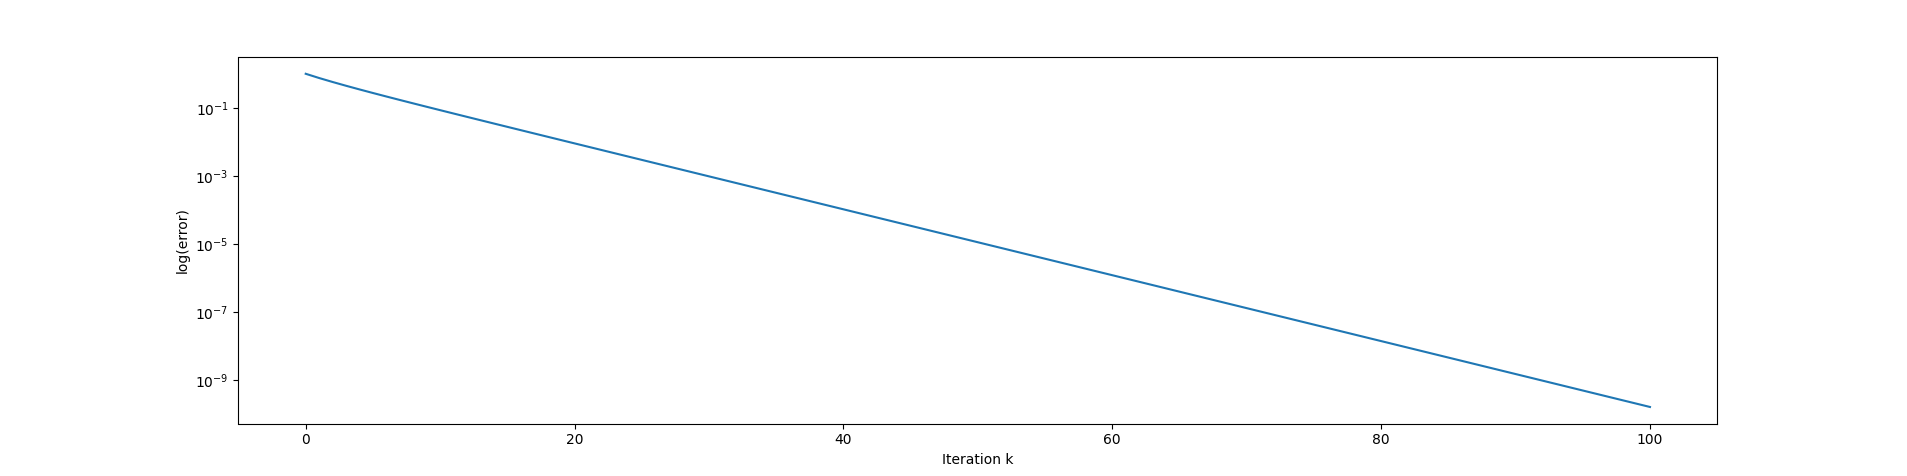
\includegraphics[width=\linewidth]{Images/newtons_plot.png}
    \captionof{figure}{Plot of errors for standard Newton's method on $(x-1)^5 e^x$}
    \label{fig:error-plot-newton}
\end{center}
\begin{center}
    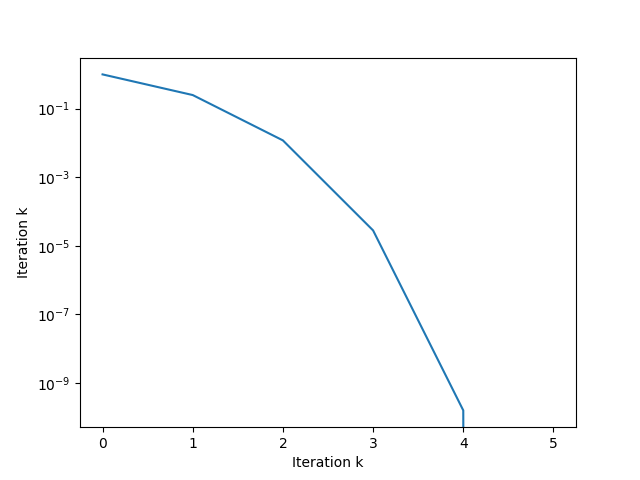
\includegraphics[width=0.8\linewidth]{Images/modified_newtons_plot.png}
    \captionof{figure}{Plot of errors for modified Newton's method on $(x-1)^5 e^x$}
    \label{fig:error-plot-modified}
\end{center}



\end{letterenum}

\section{Problem 5}

Let the first step of the secant method be given by:
\begin{equation*}
    x_2 = x_1 + f(x_1) \frac{x_1 - x_0}{f(x_1) - f(x_0)}
\end{equation*}

A straightforward computation shows that $x_0$ and $x_1$ can be swapped:
\begin{align*}
    x_2 &= x_1 \cdot \frac{f(x_1) - f(x_0)}{f(x_1) - f(x_0)} - f(x_1) \cdot 
        \frac{x_1 - x_0}{f(x_1) - f(x_0)} \\
        &= \frac{x_1 f(x_1) - x_1 f(x_0) - x_1 f(x_1) + x_0 f(x_1)}{f(x_1) - f(x_0)} \\
        &= \frac{x_0 f(x_1) - x_1 f(x_0)}{f(x_1) - f(x_0)} \\
        &= \frac{x_0 f(x_1) - x_0 f(x_0) + x_0 f(x_0) - x_1 f(x_0)}{f(x_1) - f(x_0)} \\
        &= x_0 - f(x_0) \cdot \frac{x_1 - x_0}{f(x_1) - f(x_0)} \\
        &= x_0 - f(x_0) \cdot \frac{x_0 - x_1}{f(x_0) - f(x_1)}
\end{align*}


\section{Appendix: Code}
\begin{python}
import math

import matplotlib.pyplot as plt
import numpy as np


class SolverResult:
    def __init__(self, root, success, steps):
        self.root = root
        self.success = success
        self.steps = steps


KNOWN_METHODS = ["newton", "modified_newton"]
VERY_SMALL = 1e-50

def find_root(f, f_prime, x0, tol, n_max, method="newton", root_multiplicity=None):
    """
    Find the root of the function using Newtons method.
    
    Input:
        f: function
        f_prime: derivative of f
        x0: initial guess
        tol: tolerance
        n_max: max iterations
        method: "newton" for standard newton's or "modified_newton" for modified
            version
        root_multiplicity: multiplicity of root to be used for modified method.

    outputs:
        SolverResult:
            root: found root of function
            success: True if tolerance was attained before maximum number of iterations.
            steps: x_n for each n in the iteration.
    """
    if method not in KNOWN_METHODS:
        raise ValueError(f"Unknown method: {method}. Accepted methods: {KNOWN_METHODS}")  # noqa
    if method == "modified_newton" and root_multiplicity is None:
        raise ValueError("root_multiplicity must be specified with modified newton method.") # noqa

    p = root_multiplicity

    steps = [x0]
    for _ in range(n_max):
        if method == "newton":
            x1 = x0 - f(x0) / f_prime(x0)
        elif method == "modified_newton":
            x1 = x0 - p * f(x0) / f_prime(x0)
        steps.append(x1)
        # Also add a stop condition when |f(x1)| is very small. 
        # This corresponds to the case where
        if abs(x1 - x0) < tol or abs(f(x1)) < VERY_SMALL:
            return SolverResult(x1, True, np.array(steps))
        x0 = x1
    return SolverResult(x1, False, np.array(steps))


def f(x):
    return (x - 1) ** 5 * np.exp(x)

def f_prime(x):
    return (x-1)**4 * np.exp(x) * ((x-1) + 5)

def f_pprime(x):
    return (x-1)**3 * np.exp(x) * ((x-1)**2 + 10 * (x-1) + 20)


def print_table(err, steps):
    print(f"k    x_k               Error")
    for i, (x_k, e) in enumerate(zip(steps, err)):
        if i > 20 and i %5 != 0:
            continue
        print(f"{str(i):<4}", f"{x_k:.10e}", f"{e:.10e}")

def problem_5():
    x0 = 0.001
    tol = 1e-15
    n_max = 100
    result = find_root(f, f_prime, x0, tol, n_max, "modified_newton", 5)
    err = np.abs(1 - result.steps)
    print_table(err, result.steps)

    fig = plt.figure()
    plt.semilogy(err)
    plt.xlabel("Iteration k")
    plt.ylabel("Iteration k")
    fig.savefig("tex/hw3/Images/modified_newtons_plot.png")
    plt.show()

    result = find_root(f, f_prime, x0, tol, n_max, "newton", 5)
    err = np.abs(1 - result.steps)
    print_table(err, result.steps)
    fig = plt.figure()
    plt.semilogy(err)
    plt.xlabel("Iteration k")
    plt.ylabel("log(error)")
    plt.show()
    fig.savefig("tex/hw3/Images/newtons_plot.png")

###########################################
# Bisection code from HW2
###########################################


EXIT_SUCCESS = 0
EXIT_FAILURE = 1


class BisectionResult:
    def __init__(self, root, exit_status, steps):
        self.root = root
        self.exit_status = exit_status
        self.steps = steps


def bisection(f, a, b, atol):
    steps = [a]
    fa = f(a)
    fb = f(b)
    if fa * fb > 0:
        return BisectionResult(
            a, EXIT_FAILURE, steps
        )

    while abs(a - b) > atol:
        c = 1/2 * (a + b)
        fc = f(c)
        if fa * fc < 0:
            b = c
        else:
            a = c
            fa = fc
        steps.append(a)
    return BisectionResult(
        a, EXIT_SUCCESS, steps
    )

###########################################
# Problem 2
###########################################

ALPHA = 0.138e-6  # m^2 / second
T_s = -15  # degree Celsius
T_i = 20  # degree Celsius
T0 = 60 * 3600 * 24  # seconds


def f2(x):
    return math.erf(x / 2 / math.sqrt(ALPHA * T0)) + T_s / (T_i - T_s)

def f2_prime(x):
    return 2 / math.sqrt(math.pi) * math.exp(- x**2 / 4 / ALPHA / T0)


def problem_2():
    x_bar = 10

    x = np.linspace(0, x_bar, 1000)
    fig = plt.figure()
    plt.plot(x, [f2(x_i) for x_i in x])
    plt.xlabel("Distance underground (meters)")
    plt.ylabel("f(x)")
    fig.savefig("tex/hw3/Images/temp_plot.png")
    plt.show()
    tol = 1e-13
    result = bisection(f2, 0, x_bar, tol)
    print(f"Bisection outcome = {result.exit_status}")
    print(f"root: {result.root}")
    print(f"number of iterations: {len(result.steps)}")

    x0 = 0.01
    newton_result = find_root(f2, f2_prime, x0, tol, 100)
    print("With x0=0.01")
    print(f"Newton converged:  {newton_result.success}")
    print(f"Newton root:  {newton_result.root}")
    print(f"number of iterations: {len(newton_result.steps)}")

    x0 = x_bar
    newton_result = find_root(f2, f2_prime, x0, tol, 100)
    print("With x0=0.01")
    print(f"Newton converged:  {newton_result.success}")
    print(f"Newton root:  {newton_result.root}")
    print(f"number of iterations: {len(newton_result.steps)}")

if __name__ == '__main__':
    problem_5()


\end{python}




\end{document}
